% !TEX root = Bachelorarbeit_Paul_Zilewitsch.tex

\begin{flushright}
Anhang 1\\
Blatt 1\\
\end{flushright}

\begin{figure}[h!]
\centering
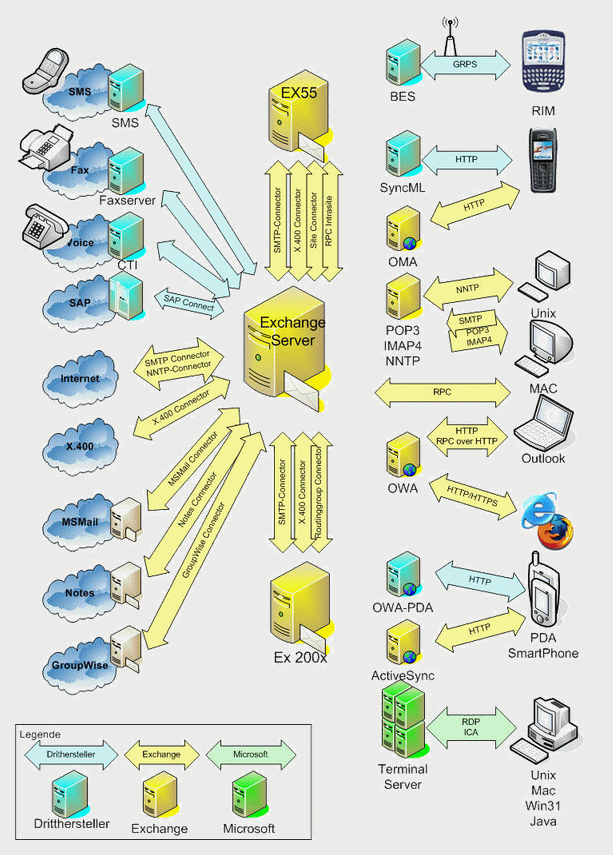
\includegraphics[width=0.70\textwidth]{Abbildungen/Exchange_Verbindungen.png}
\caption*{\\Exchange Verbindungen, Quelle: http://www.msxfaq.de/basics/excomm.htm}
\label{Exchange_Verbindungen}
\end{figure}


\newpage

\begin{flushright}
Anhang 2\\
Blatt 1\\
\end{flushright}

\begin{figure}[h!]
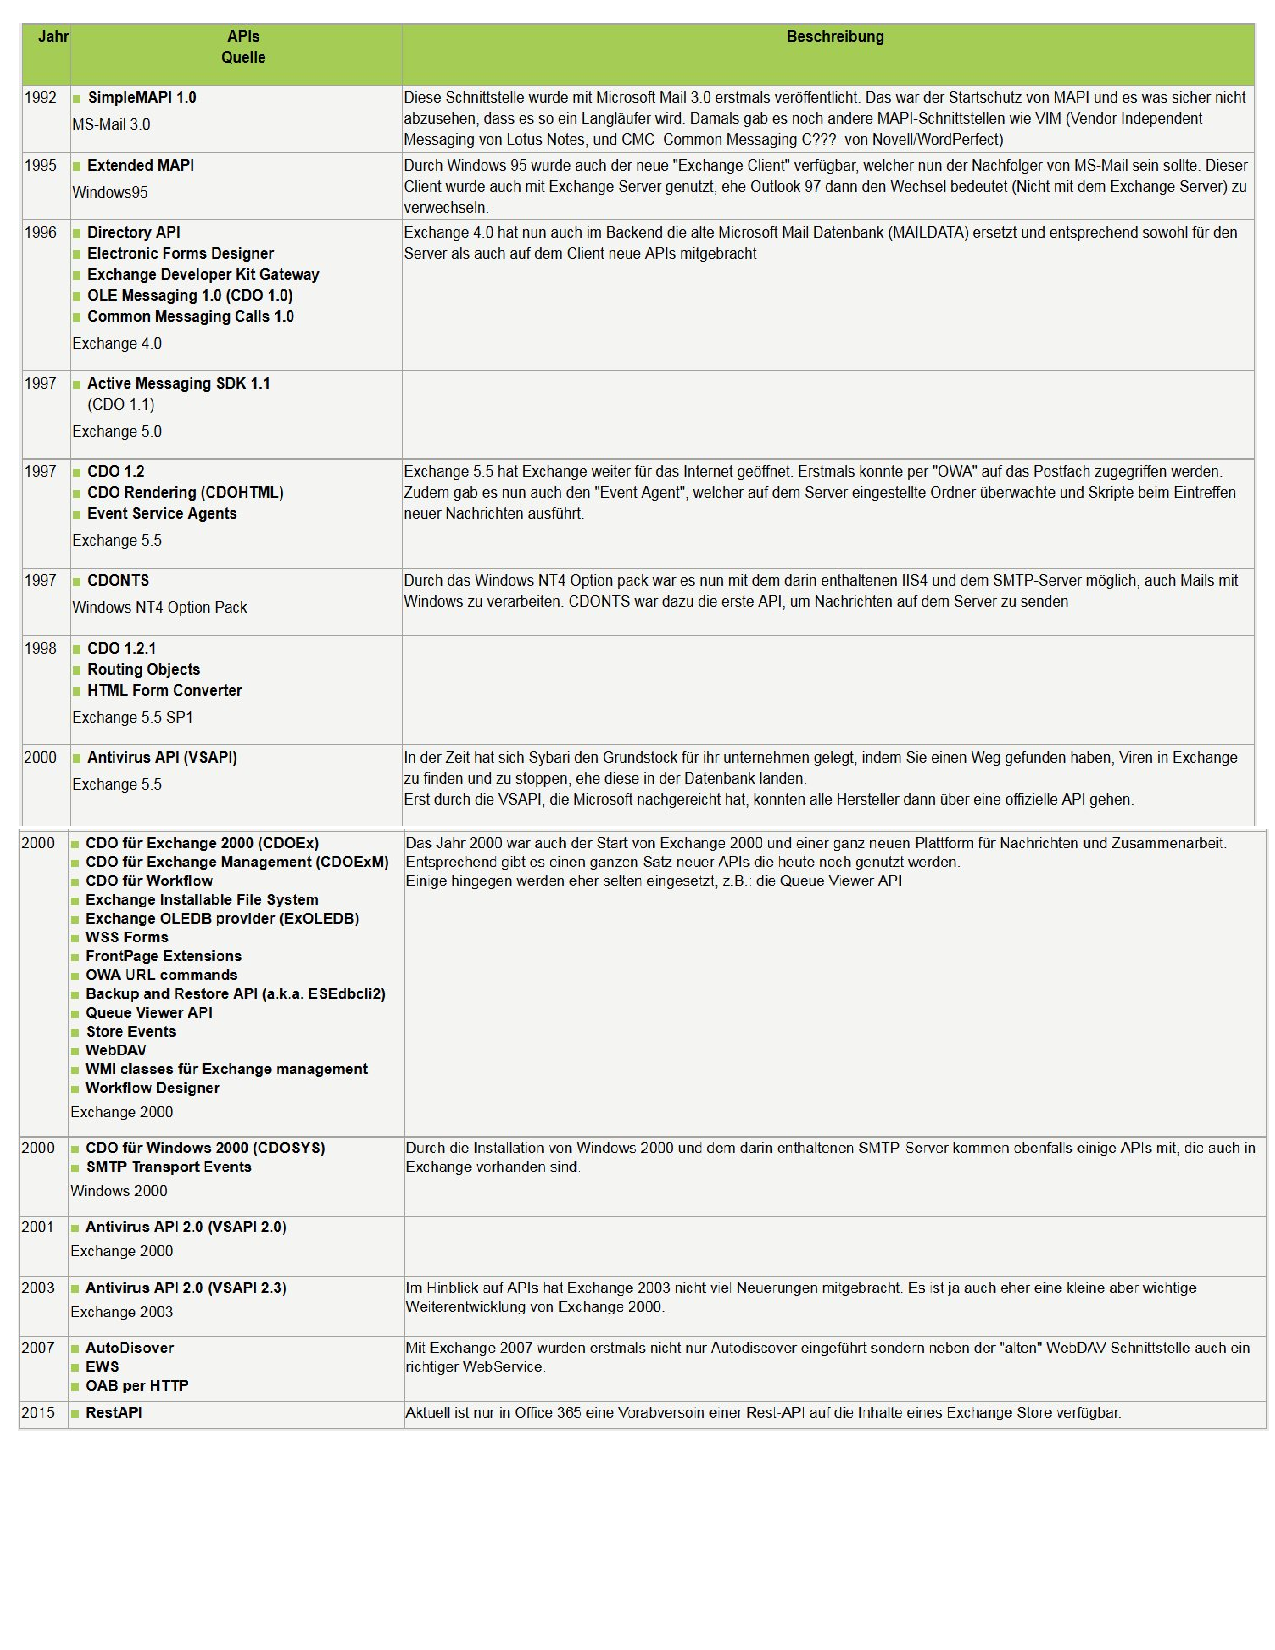
\includegraphics[width=1.0\textwidth]{Abbildungen/API_Geschichte2.pdf}
\caption*{Geschichte der APIs, Quelle: http://www.msxfaq.de/code/wege.htm}
\label{API_Geschichte}
\end{figure}

\newpage

\begin{flushright}
Anhang 3\\
Blatt 1\\
\label{Anhang3_1}
\end{flushright}

\begin{figure}[h!]
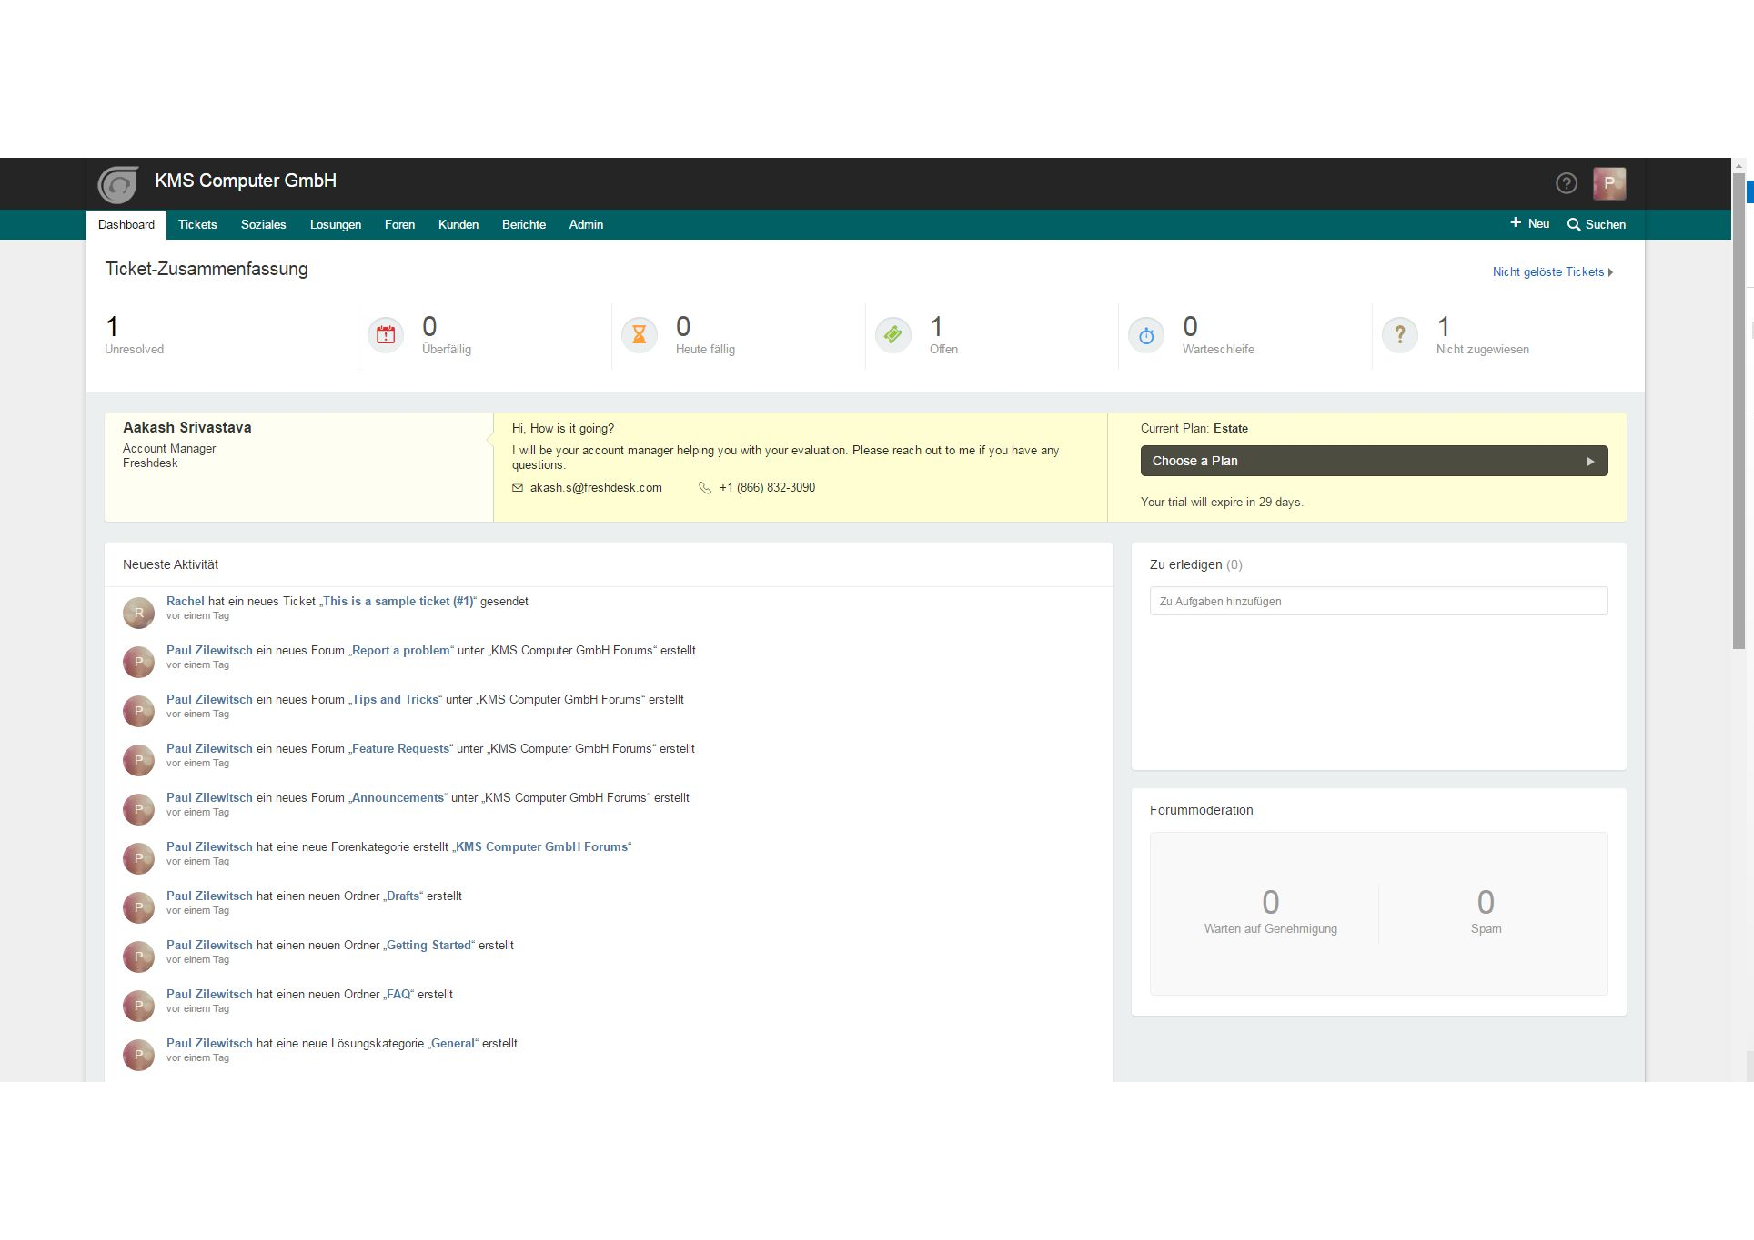
\includegraphics[width=0.85\textwidth]{Abbildungen/Freshdesk.pdf}
\caption*{Screenshot Freshdesk Dashboard, \newline
Quelle: https://kmscomputergmbh.freshdesk.com/helpdesk/dashboard}
\label{Freshdesk}
\end{figure}



\begin{figure}[h!]
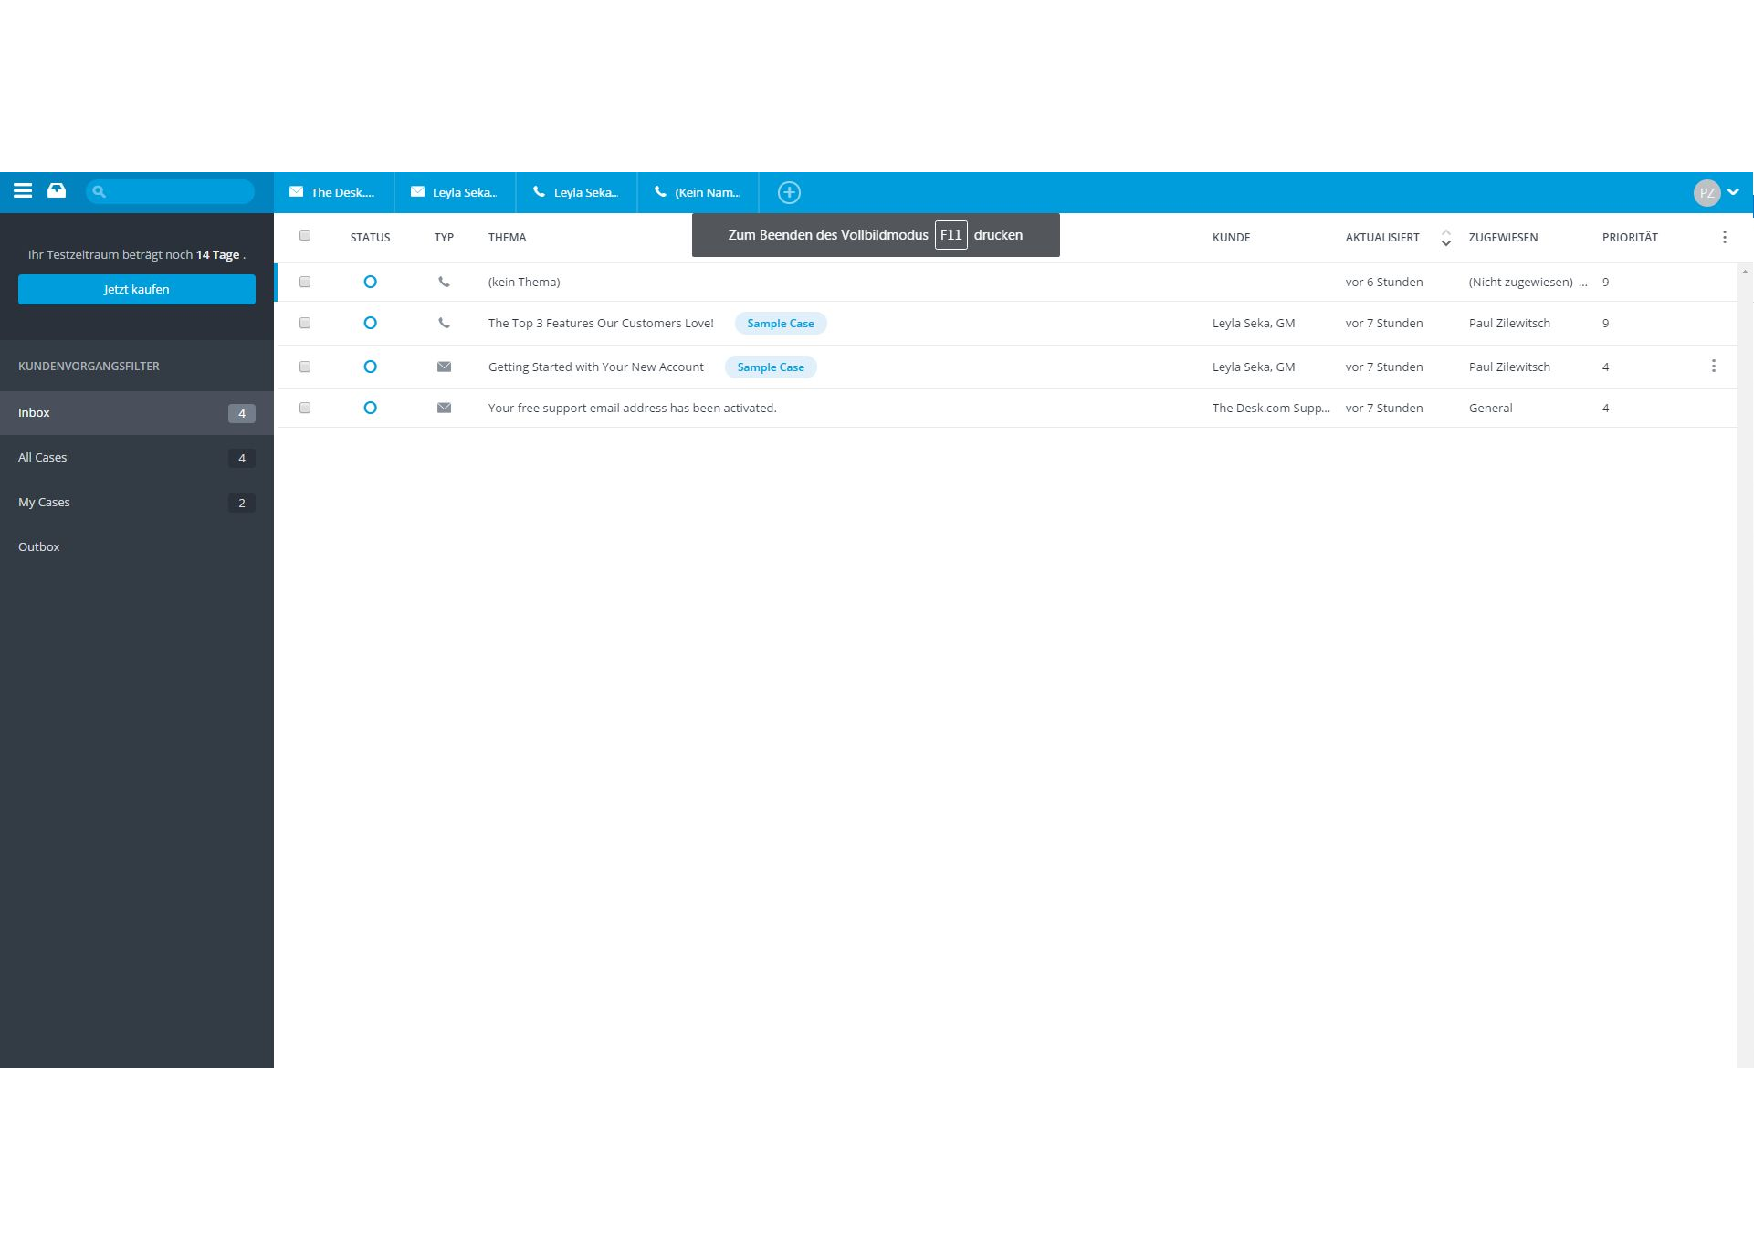
\includegraphics[width=0.85\textwidth]{Abbildungen/Deskcom.pdf}
\caption*{Screenshot Desk.com Dashboard,Quelle: https://kmscomputergmbh.desk.com/web/agent}
\label{Deskcom}
\end{figure}

\newpage

\begin{flushright}
Anhang 3\\
Blatt 2\\
\label{Anhang3_2}
\end{flushright}


\begin{figure}[h!]
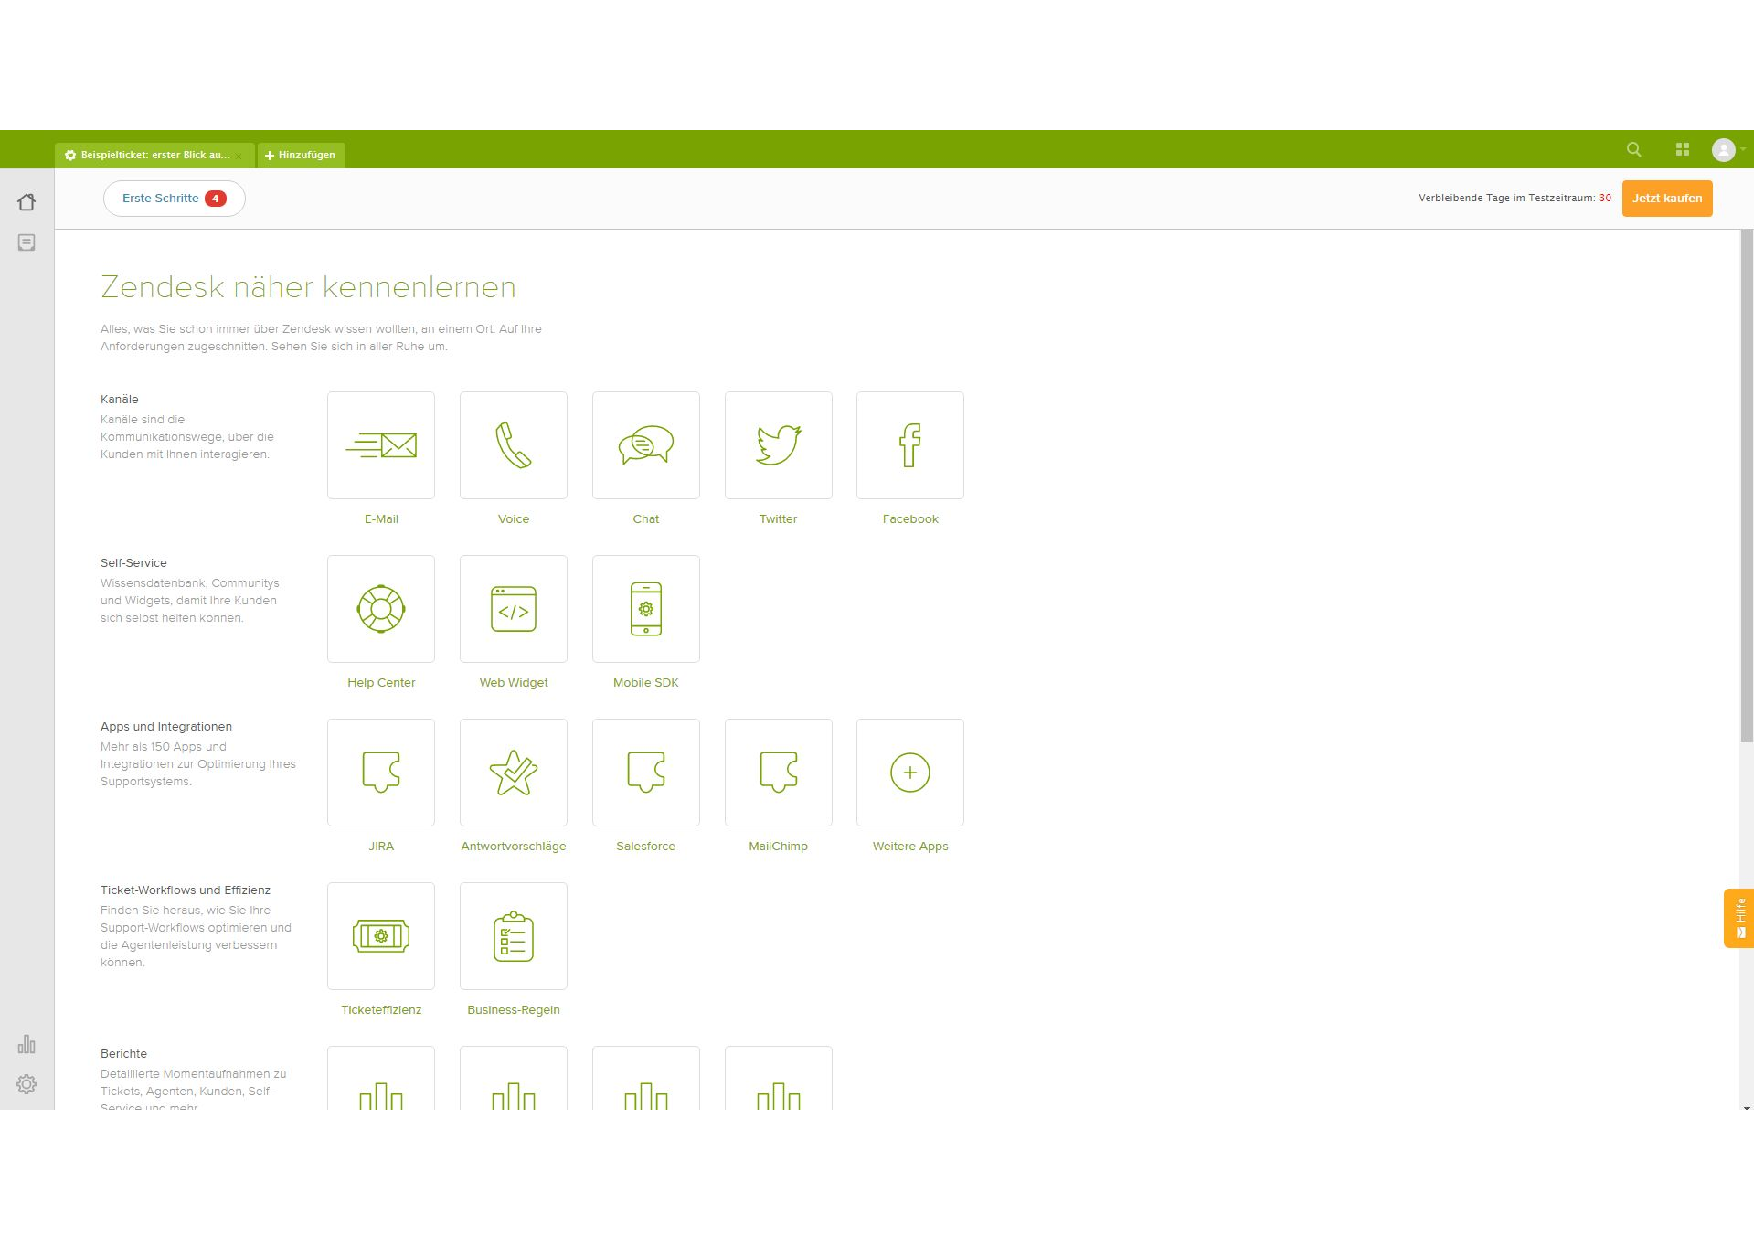
\includegraphics[width=0.85\textwidth]{Abbildungen/Zendesk.pdf}
\caption*{Screenshot Zendesk Dashboard, \newline
Quelle: https://kmscomputergmbh.zendesk.com/agent/discovery}
\label{Zendesk}
\end{figure}

\begin{figure}[h!]
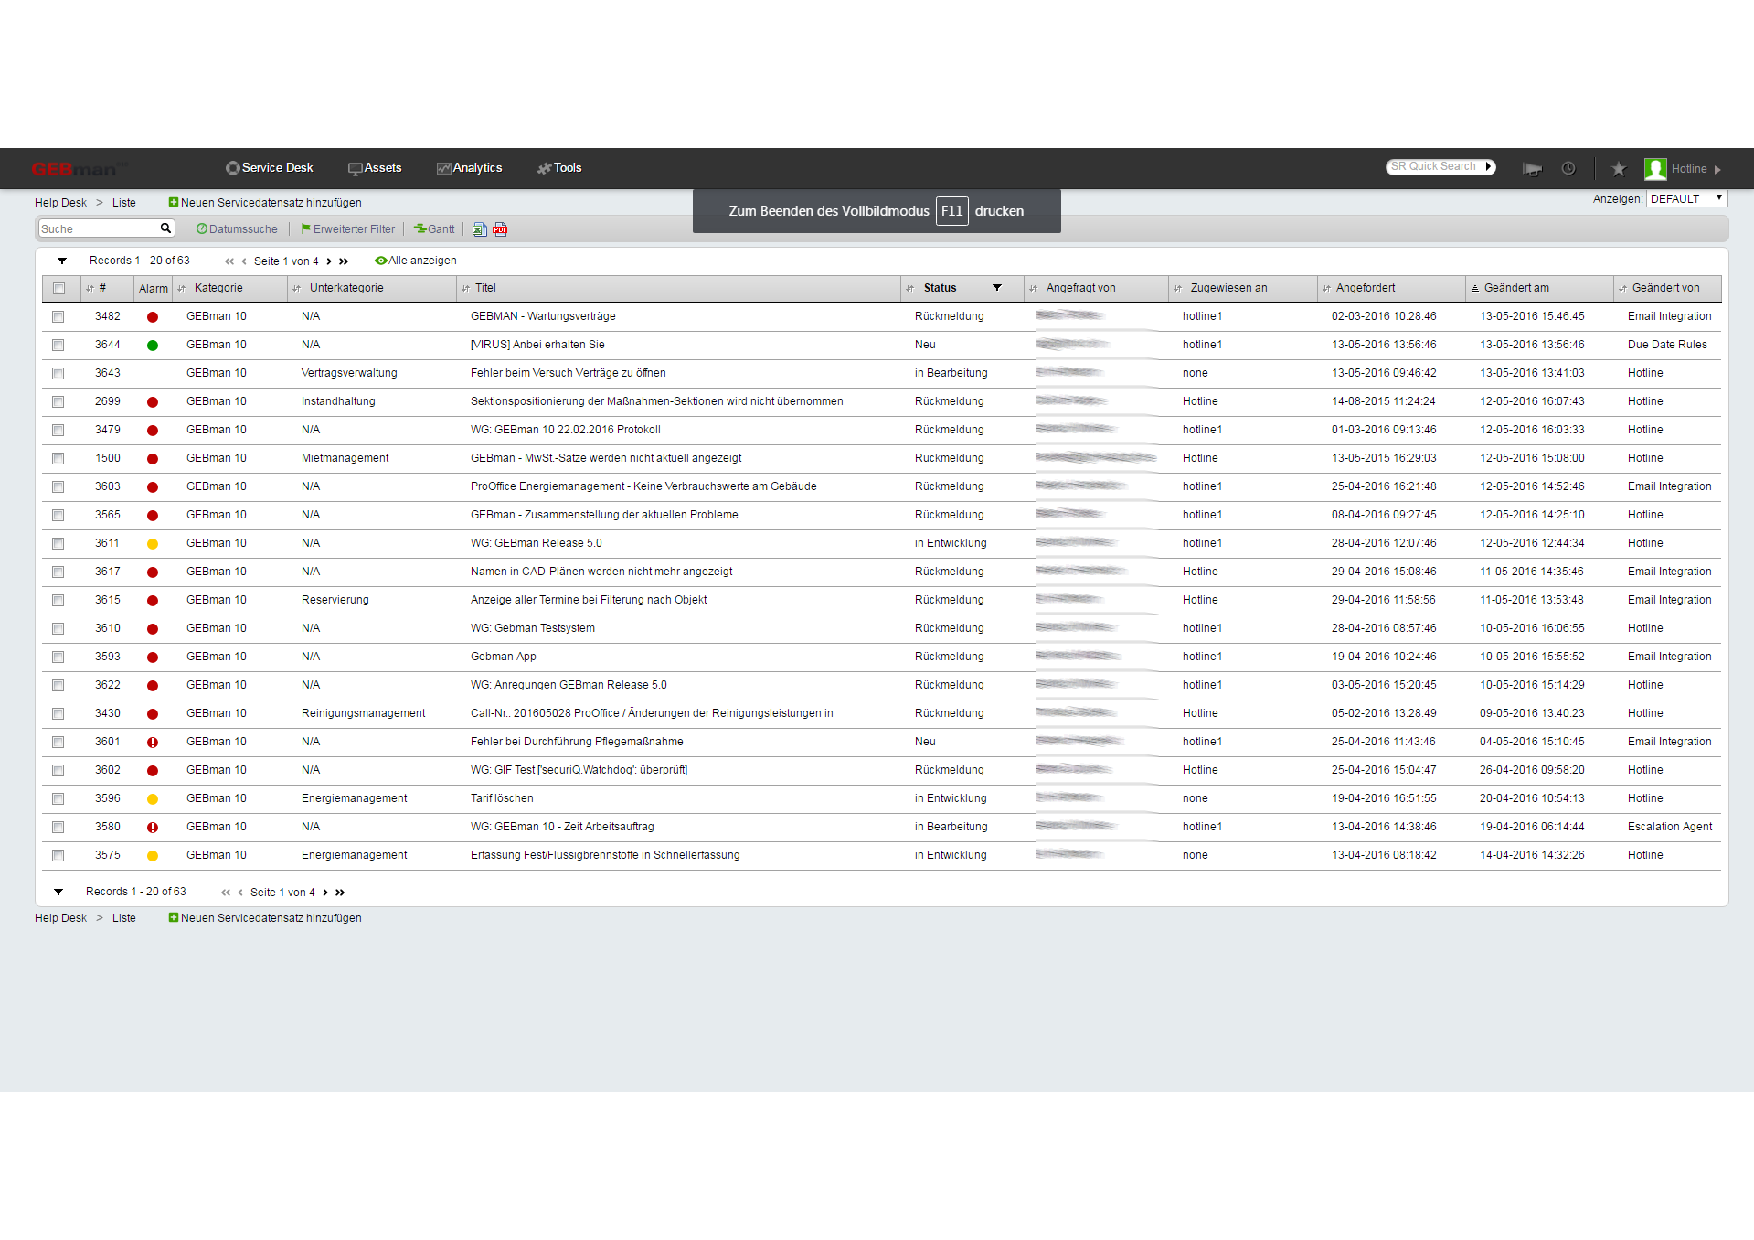
\includegraphics[width=0.85\textwidth]{Abbildungen/SysAid.pdf}
\caption*{Screenshot SysAid Dashboard, \newline
Quelle: http://gebmanhelp.gebman.com:8080/HelpDesk.jsp?helpdeskfrm\&fromId\=List}
\label{SysAid}
\end{figure}

\newpage


\begin{flushright}
Anhang 4\\
Blatt 1\\
\label{Anhang4}
\end{flushright}


\begin{figure}[h!]
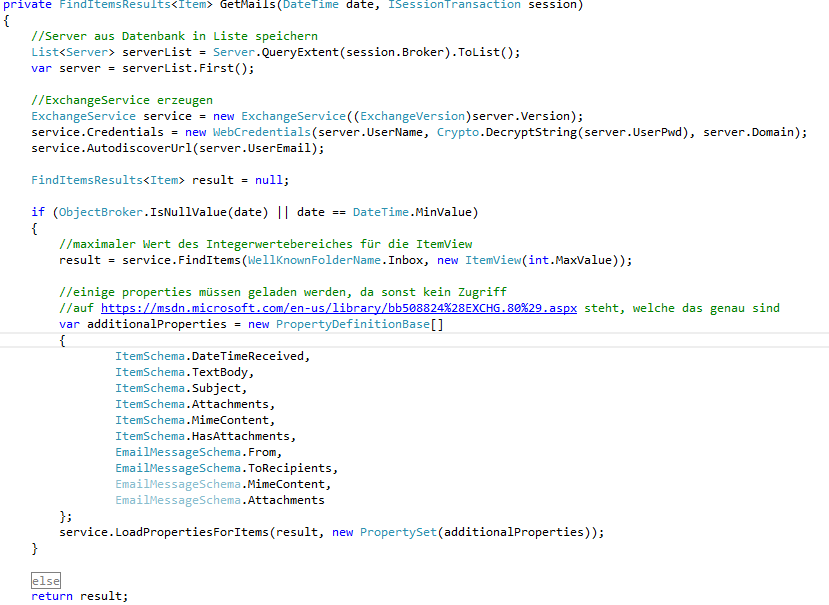
\includegraphics[width=0.9\textwidth]{Abbildungen/Codeausschnitt.png}
	\caption*{Codeausschnitt \textit{GetMails( )}, Quelle: eigene Darstellung}
	\label{Codeausschnitt}
\end{figure}







